\section{APPLICATION TO SCALE FREE NETWORK WITH FRACTIONAL ORDER DYNAMICS}
\label{sec:scalefree}

In \cite{goodwinemed2023,goodwinemmar2023} we studied the effects of various
parameters in large, scale free networks on the existence of fractional order
dynamics. To further validate the generalizability of the results for the neural
network, we apply it to a large, scale free network with fractional order
dynamics.

Specifically, we consider a network with 2000 nodes. Each node has a mass of 1
and is connected to various other nodes with either a spring or damper, with
coefficients $k = 2501$ and $b = 150$. The details of the manner in which the
network is constructed to make it scale free are contained in the references.
The step response of the system when one of the masses has a non-zero initial
condition is computed, and the response of one of the nodes is observed. The
network used for this validation is illustrated in Figure~\ref{fig:network} and
the response of node 1011 when node 100 was displaced by 1 was determined by
numerically solving the system of 4000 first order differential equations and is
illustrated in Figure~\ref{fig:sfresp}..

\begin{figure}
\centering
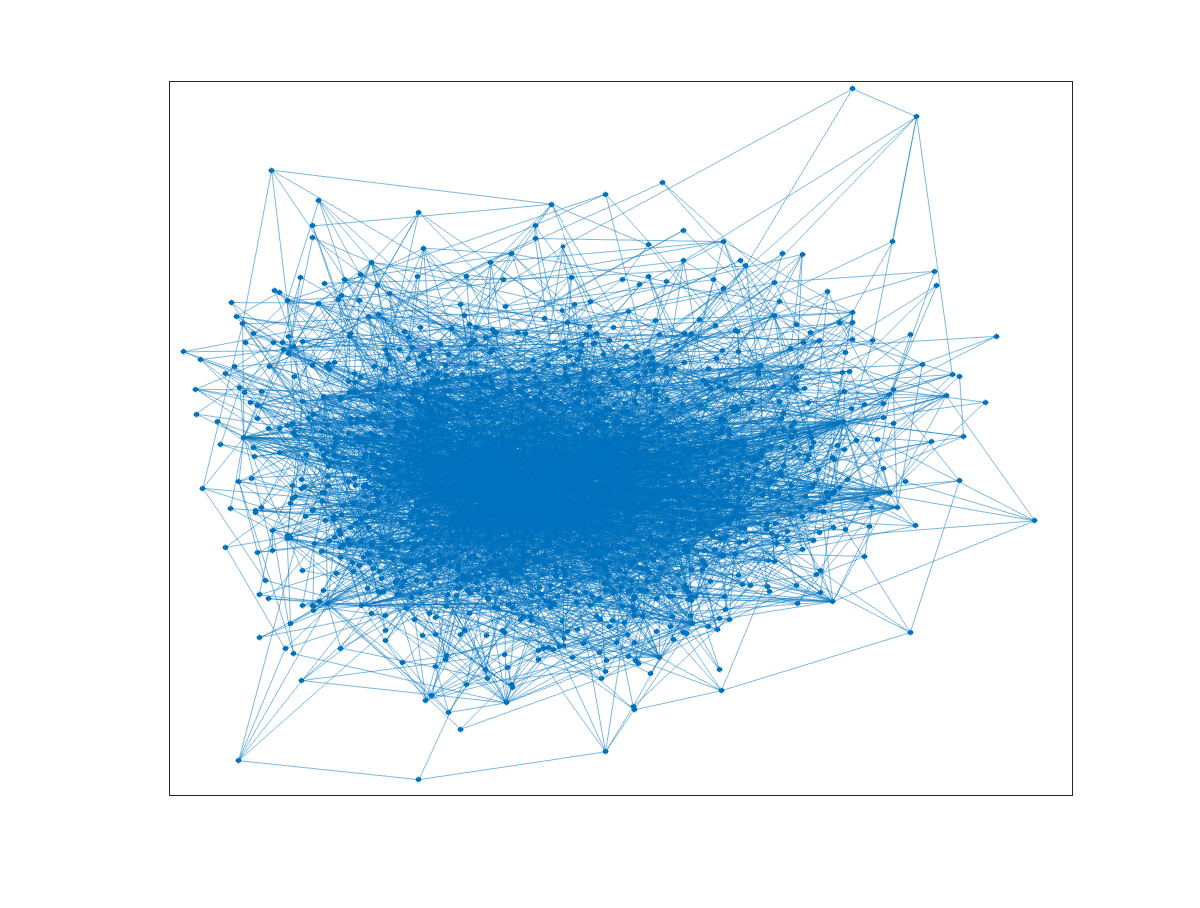
\includegraphics[width=3.5in]{network}
\caption{Large scale free network used for validation.}
\label{fig:network}
\end{figure}

\begin{figure}
\centering
%% Creator: Matplotlib, PGF backend
%%
%% To include the figure in your LaTeX document, write
%%   \input{<filename>.pgf}
%%
%% Make sure the required packages are loaded in your preamble
%%   \usepackage{pgf}
%%
%% Also ensure that all the required font packages are loaded; for instance,
%% the lmodern package is sometimes necessary when using math font.
%%   \usepackage{lmodern}
%%
%% Figures using additional raster images can only be included by \input if
%% they are in the same directory as the main LaTeX file. For loading figures
%% from other directories you can use the `import` package
%%   \usepackage{import}
%%
%% and then include the figures with
%%   \import{<path to file>}{<filename>.pgf}
%%
%% Matplotlib used the following preamble
%%   \def\mathdefault#1{#1}
%%   \everymath=\expandafter{\the\everymath\displaystyle}
%%   
%%   \usepackage{fontspec}
%%   \setmainfont{DejaVuSerif.ttf}[Path=\detokenize{/Users/billgoodwine/research/step/steps/lib/python3.11/site-packages/matplotlib/mpl-data/fonts/ttf/}]
%%   \setsansfont{DejaVuSans.ttf}[Path=\detokenize{/Users/billgoodwine/research/step/steps/lib/python3.11/site-packages/matplotlib/mpl-data/fonts/ttf/}]
%%   \setmonofont{DejaVuSansMono.ttf}[Path=\detokenize{/Users/billgoodwine/research/step/steps/lib/python3.11/site-packages/matplotlib/mpl-data/fonts/ttf/}]
%%   \makeatletter\@ifpackageloaded{underscore}{}{\usepackage[strings]{underscore}}\makeatother
%%
\begingroup%
\makeatletter%
\begin{pgfpicture}%
\pgfpathrectangle{\pgfpointorigin}{\pgfqpoint{3.500000in}{2.379431in}}%
\pgfusepath{use as bounding box, clip}%
\begin{pgfscope}%
\pgfsetbuttcap%
\pgfsetmiterjoin%
\definecolor{currentfill}{rgb}{1.000000,1.000000,1.000000}%
\pgfsetfillcolor{currentfill}%
\pgfsetlinewidth{0.000000pt}%
\definecolor{currentstroke}{rgb}{1.000000,1.000000,1.000000}%
\pgfsetstrokecolor{currentstroke}%
\pgfsetdash{}{0pt}%
\pgfpathmoveto{\pgfqpoint{0.000000in}{0.000000in}}%
\pgfpathlineto{\pgfqpoint{3.500000in}{0.000000in}}%
\pgfpathlineto{\pgfqpoint{3.500000in}{2.379431in}}%
\pgfpathlineto{\pgfqpoint{0.000000in}{2.379431in}}%
\pgfpathlineto{\pgfqpoint{0.000000in}{0.000000in}}%
\pgfpathclose%
\pgfusepath{fill}%
\end{pgfscope}%
\begin{pgfscope}%
\pgfsetbuttcap%
\pgfsetmiterjoin%
\definecolor{currentfill}{rgb}{1.000000,1.000000,1.000000}%
\pgfsetfillcolor{currentfill}%
\pgfsetlinewidth{0.000000pt}%
\definecolor{currentstroke}{rgb}{0.000000,0.000000,0.000000}%
\pgfsetstrokecolor{currentstroke}%
\pgfsetstrokeopacity{0.000000}%
\pgfsetdash{}{0pt}%
\pgfpathmoveto{\pgfqpoint{0.619136in}{0.571603in}}%
\pgfpathlineto{\pgfqpoint{3.350000in}{0.571603in}}%
\pgfpathlineto{\pgfqpoint{3.350000in}{2.229431in}}%
\pgfpathlineto{\pgfqpoint{0.619136in}{2.229431in}}%
\pgfpathlineto{\pgfqpoint{0.619136in}{0.571603in}}%
\pgfpathclose%
\pgfusepath{fill}%
\end{pgfscope}%
\begin{pgfscope}%
\pgfpathrectangle{\pgfqpoint{0.619136in}{0.571603in}}{\pgfqpoint{2.730864in}{1.657828in}}%
\pgfusepath{clip}%
\pgfsetrectcap%
\pgfsetroundjoin%
\pgfsetlinewidth{0.803000pt}%
\definecolor{currentstroke}{rgb}{0.690196,0.690196,0.690196}%
\pgfsetstrokecolor{currentstroke}%
\pgfsetdash{}{0pt}%
\pgfpathmoveto{\pgfqpoint{0.743267in}{0.571603in}}%
\pgfpathlineto{\pgfqpoint{0.743267in}{2.229431in}}%
\pgfusepath{stroke}%
\end{pgfscope}%
\begin{pgfscope}%
\pgfsetbuttcap%
\pgfsetroundjoin%
\definecolor{currentfill}{rgb}{0.000000,0.000000,0.000000}%
\pgfsetfillcolor{currentfill}%
\pgfsetlinewidth{0.803000pt}%
\definecolor{currentstroke}{rgb}{0.000000,0.000000,0.000000}%
\pgfsetstrokecolor{currentstroke}%
\pgfsetdash{}{0pt}%
\pgfsys@defobject{currentmarker}{\pgfqpoint{0.000000in}{-0.048611in}}{\pgfqpoint{0.000000in}{0.000000in}}{%
\pgfpathmoveto{\pgfqpoint{0.000000in}{0.000000in}}%
\pgfpathlineto{\pgfqpoint{0.000000in}{-0.048611in}}%
\pgfusepath{stroke,fill}%
}%
\begin{pgfscope}%
\pgfsys@transformshift{0.743267in}{0.571603in}%
\pgfsys@useobject{currentmarker}{}%
\end{pgfscope}%
\end{pgfscope}%
\begin{pgfscope}%
\definecolor{textcolor}{rgb}{0.000000,0.000000,0.000000}%
\pgfsetstrokecolor{textcolor}%
\pgfsetfillcolor{textcolor}%
\pgftext[x=0.743267in,y=0.474381in,,top]{\color{textcolor}{\rmfamily\fontsize{10.000000}{12.000000}\selectfont\catcode`\^=\active\def^{\ifmmode\sp\else\^{}\fi}\catcode`\%=\active\def%{\%}$\mathdefault{0}$}}%
\end{pgfscope}%
\begin{pgfscope}%
\pgfpathrectangle{\pgfqpoint{0.619136in}{0.571603in}}{\pgfqpoint{2.730864in}{1.657828in}}%
\pgfusepath{clip}%
\pgfsetrectcap%
\pgfsetroundjoin%
\pgfsetlinewidth{0.803000pt}%
\definecolor{currentstroke}{rgb}{0.690196,0.690196,0.690196}%
\pgfsetstrokecolor{currentstroke}%
\pgfsetdash{}{0pt}%
\pgfpathmoveto{\pgfqpoint{1.239787in}{0.571603in}}%
\pgfpathlineto{\pgfqpoint{1.239787in}{2.229431in}}%
\pgfusepath{stroke}%
\end{pgfscope}%
\begin{pgfscope}%
\pgfsetbuttcap%
\pgfsetroundjoin%
\definecolor{currentfill}{rgb}{0.000000,0.000000,0.000000}%
\pgfsetfillcolor{currentfill}%
\pgfsetlinewidth{0.803000pt}%
\definecolor{currentstroke}{rgb}{0.000000,0.000000,0.000000}%
\pgfsetstrokecolor{currentstroke}%
\pgfsetdash{}{0pt}%
\pgfsys@defobject{currentmarker}{\pgfqpoint{0.000000in}{-0.048611in}}{\pgfqpoint{0.000000in}{0.000000in}}{%
\pgfpathmoveto{\pgfqpoint{0.000000in}{0.000000in}}%
\pgfpathlineto{\pgfqpoint{0.000000in}{-0.048611in}}%
\pgfusepath{stroke,fill}%
}%
\begin{pgfscope}%
\pgfsys@transformshift{1.239787in}{0.571603in}%
\pgfsys@useobject{currentmarker}{}%
\end{pgfscope}%
\end{pgfscope}%
\begin{pgfscope}%
\definecolor{textcolor}{rgb}{0.000000,0.000000,0.000000}%
\pgfsetstrokecolor{textcolor}%
\pgfsetfillcolor{textcolor}%
\pgftext[x=1.239787in,y=0.474381in,,top]{\color{textcolor}{\rmfamily\fontsize{10.000000}{12.000000}\selectfont\catcode`\^=\active\def^{\ifmmode\sp\else\^{}\fi}\catcode`\%=\active\def%{\%}$\mathdefault{2}$}}%
\end{pgfscope}%
\begin{pgfscope}%
\pgfpathrectangle{\pgfqpoint{0.619136in}{0.571603in}}{\pgfqpoint{2.730864in}{1.657828in}}%
\pgfusepath{clip}%
\pgfsetrectcap%
\pgfsetroundjoin%
\pgfsetlinewidth{0.803000pt}%
\definecolor{currentstroke}{rgb}{0.690196,0.690196,0.690196}%
\pgfsetstrokecolor{currentstroke}%
\pgfsetdash{}{0pt}%
\pgfpathmoveto{\pgfqpoint{1.736308in}{0.571603in}}%
\pgfpathlineto{\pgfqpoint{1.736308in}{2.229431in}}%
\pgfusepath{stroke}%
\end{pgfscope}%
\begin{pgfscope}%
\pgfsetbuttcap%
\pgfsetroundjoin%
\definecolor{currentfill}{rgb}{0.000000,0.000000,0.000000}%
\pgfsetfillcolor{currentfill}%
\pgfsetlinewidth{0.803000pt}%
\definecolor{currentstroke}{rgb}{0.000000,0.000000,0.000000}%
\pgfsetstrokecolor{currentstroke}%
\pgfsetdash{}{0pt}%
\pgfsys@defobject{currentmarker}{\pgfqpoint{0.000000in}{-0.048611in}}{\pgfqpoint{0.000000in}{0.000000in}}{%
\pgfpathmoveto{\pgfqpoint{0.000000in}{0.000000in}}%
\pgfpathlineto{\pgfqpoint{0.000000in}{-0.048611in}}%
\pgfusepath{stroke,fill}%
}%
\begin{pgfscope}%
\pgfsys@transformshift{1.736308in}{0.571603in}%
\pgfsys@useobject{currentmarker}{}%
\end{pgfscope}%
\end{pgfscope}%
\begin{pgfscope}%
\definecolor{textcolor}{rgb}{0.000000,0.000000,0.000000}%
\pgfsetstrokecolor{textcolor}%
\pgfsetfillcolor{textcolor}%
\pgftext[x=1.736308in,y=0.474381in,,top]{\color{textcolor}{\rmfamily\fontsize{10.000000}{12.000000}\selectfont\catcode`\^=\active\def^{\ifmmode\sp\else\^{}\fi}\catcode`\%=\active\def%{\%}$\mathdefault{4}$}}%
\end{pgfscope}%
\begin{pgfscope}%
\pgfpathrectangle{\pgfqpoint{0.619136in}{0.571603in}}{\pgfqpoint{2.730864in}{1.657828in}}%
\pgfusepath{clip}%
\pgfsetrectcap%
\pgfsetroundjoin%
\pgfsetlinewidth{0.803000pt}%
\definecolor{currentstroke}{rgb}{0.690196,0.690196,0.690196}%
\pgfsetstrokecolor{currentstroke}%
\pgfsetdash{}{0pt}%
\pgfpathmoveto{\pgfqpoint{2.232829in}{0.571603in}}%
\pgfpathlineto{\pgfqpoint{2.232829in}{2.229431in}}%
\pgfusepath{stroke}%
\end{pgfscope}%
\begin{pgfscope}%
\pgfsetbuttcap%
\pgfsetroundjoin%
\definecolor{currentfill}{rgb}{0.000000,0.000000,0.000000}%
\pgfsetfillcolor{currentfill}%
\pgfsetlinewidth{0.803000pt}%
\definecolor{currentstroke}{rgb}{0.000000,0.000000,0.000000}%
\pgfsetstrokecolor{currentstroke}%
\pgfsetdash{}{0pt}%
\pgfsys@defobject{currentmarker}{\pgfqpoint{0.000000in}{-0.048611in}}{\pgfqpoint{0.000000in}{0.000000in}}{%
\pgfpathmoveto{\pgfqpoint{0.000000in}{0.000000in}}%
\pgfpathlineto{\pgfqpoint{0.000000in}{-0.048611in}}%
\pgfusepath{stroke,fill}%
}%
\begin{pgfscope}%
\pgfsys@transformshift{2.232829in}{0.571603in}%
\pgfsys@useobject{currentmarker}{}%
\end{pgfscope}%
\end{pgfscope}%
\begin{pgfscope}%
\definecolor{textcolor}{rgb}{0.000000,0.000000,0.000000}%
\pgfsetstrokecolor{textcolor}%
\pgfsetfillcolor{textcolor}%
\pgftext[x=2.232829in,y=0.474381in,,top]{\color{textcolor}{\rmfamily\fontsize{10.000000}{12.000000}\selectfont\catcode`\^=\active\def^{\ifmmode\sp\else\^{}\fi}\catcode`\%=\active\def%{\%}$\mathdefault{6}$}}%
\end{pgfscope}%
\begin{pgfscope}%
\pgfpathrectangle{\pgfqpoint{0.619136in}{0.571603in}}{\pgfqpoint{2.730864in}{1.657828in}}%
\pgfusepath{clip}%
\pgfsetrectcap%
\pgfsetroundjoin%
\pgfsetlinewidth{0.803000pt}%
\definecolor{currentstroke}{rgb}{0.690196,0.690196,0.690196}%
\pgfsetstrokecolor{currentstroke}%
\pgfsetdash{}{0pt}%
\pgfpathmoveto{\pgfqpoint{2.729349in}{0.571603in}}%
\pgfpathlineto{\pgfqpoint{2.729349in}{2.229431in}}%
\pgfusepath{stroke}%
\end{pgfscope}%
\begin{pgfscope}%
\pgfsetbuttcap%
\pgfsetroundjoin%
\definecolor{currentfill}{rgb}{0.000000,0.000000,0.000000}%
\pgfsetfillcolor{currentfill}%
\pgfsetlinewidth{0.803000pt}%
\definecolor{currentstroke}{rgb}{0.000000,0.000000,0.000000}%
\pgfsetstrokecolor{currentstroke}%
\pgfsetdash{}{0pt}%
\pgfsys@defobject{currentmarker}{\pgfqpoint{0.000000in}{-0.048611in}}{\pgfqpoint{0.000000in}{0.000000in}}{%
\pgfpathmoveto{\pgfqpoint{0.000000in}{0.000000in}}%
\pgfpathlineto{\pgfqpoint{0.000000in}{-0.048611in}}%
\pgfusepath{stroke,fill}%
}%
\begin{pgfscope}%
\pgfsys@transformshift{2.729349in}{0.571603in}%
\pgfsys@useobject{currentmarker}{}%
\end{pgfscope}%
\end{pgfscope}%
\begin{pgfscope}%
\definecolor{textcolor}{rgb}{0.000000,0.000000,0.000000}%
\pgfsetstrokecolor{textcolor}%
\pgfsetfillcolor{textcolor}%
\pgftext[x=2.729349in,y=0.474381in,,top]{\color{textcolor}{\rmfamily\fontsize{10.000000}{12.000000}\selectfont\catcode`\^=\active\def^{\ifmmode\sp\else\^{}\fi}\catcode`\%=\active\def%{\%}$\mathdefault{8}$}}%
\end{pgfscope}%
\begin{pgfscope}%
\pgfpathrectangle{\pgfqpoint{0.619136in}{0.571603in}}{\pgfqpoint{2.730864in}{1.657828in}}%
\pgfusepath{clip}%
\pgfsetrectcap%
\pgfsetroundjoin%
\pgfsetlinewidth{0.803000pt}%
\definecolor{currentstroke}{rgb}{0.690196,0.690196,0.690196}%
\pgfsetstrokecolor{currentstroke}%
\pgfsetdash{}{0pt}%
\pgfpathmoveto{\pgfqpoint{3.225870in}{0.571603in}}%
\pgfpathlineto{\pgfqpoint{3.225870in}{2.229431in}}%
\pgfusepath{stroke}%
\end{pgfscope}%
\begin{pgfscope}%
\pgfsetbuttcap%
\pgfsetroundjoin%
\definecolor{currentfill}{rgb}{0.000000,0.000000,0.000000}%
\pgfsetfillcolor{currentfill}%
\pgfsetlinewidth{0.803000pt}%
\definecolor{currentstroke}{rgb}{0.000000,0.000000,0.000000}%
\pgfsetstrokecolor{currentstroke}%
\pgfsetdash{}{0pt}%
\pgfsys@defobject{currentmarker}{\pgfqpoint{0.000000in}{-0.048611in}}{\pgfqpoint{0.000000in}{0.000000in}}{%
\pgfpathmoveto{\pgfqpoint{0.000000in}{0.000000in}}%
\pgfpathlineto{\pgfqpoint{0.000000in}{-0.048611in}}%
\pgfusepath{stroke,fill}%
}%
\begin{pgfscope}%
\pgfsys@transformshift{3.225870in}{0.571603in}%
\pgfsys@useobject{currentmarker}{}%
\end{pgfscope}%
\end{pgfscope}%
\begin{pgfscope}%
\definecolor{textcolor}{rgb}{0.000000,0.000000,0.000000}%
\pgfsetstrokecolor{textcolor}%
\pgfsetfillcolor{textcolor}%
\pgftext[x=3.225870in,y=0.474381in,,top]{\color{textcolor}{\rmfamily\fontsize{10.000000}{12.000000}\selectfont\catcode`\^=\active\def^{\ifmmode\sp\else\^{}\fi}\catcode`\%=\active\def%{\%}$\mathdefault{10}$}}%
\end{pgfscope}%
\begin{pgfscope}%
\definecolor{textcolor}{rgb}{0.000000,0.000000,0.000000}%
\pgfsetstrokecolor{textcolor}%
\pgfsetfillcolor{textcolor}%
\pgftext[x=1.984568in,y=0.284413in,,top]{\color{textcolor}{\rmfamily\fontsize{10.000000}{12.000000}\selectfont\catcode`\^=\active\def^{\ifmmode\sp\else\^{}\fi}\catcode`\%=\active\def%{\%}$t$}}%
\end{pgfscope}%
\begin{pgfscope}%
\pgfpathrectangle{\pgfqpoint{0.619136in}{0.571603in}}{\pgfqpoint{2.730864in}{1.657828in}}%
\pgfusepath{clip}%
\pgfsetrectcap%
\pgfsetroundjoin%
\pgfsetlinewidth{0.803000pt}%
\definecolor{currentstroke}{rgb}{0.690196,0.690196,0.690196}%
\pgfsetstrokecolor{currentstroke}%
\pgfsetdash{}{0pt}%
\pgfpathmoveto{\pgfqpoint{0.619136in}{0.646959in}}%
\pgfpathlineto{\pgfqpoint{3.350000in}{0.646959in}}%
\pgfusepath{stroke}%
\end{pgfscope}%
\begin{pgfscope}%
\pgfsetbuttcap%
\pgfsetroundjoin%
\definecolor{currentfill}{rgb}{0.000000,0.000000,0.000000}%
\pgfsetfillcolor{currentfill}%
\pgfsetlinewidth{0.803000pt}%
\definecolor{currentstroke}{rgb}{0.000000,0.000000,0.000000}%
\pgfsetstrokecolor{currentstroke}%
\pgfsetdash{}{0pt}%
\pgfsys@defobject{currentmarker}{\pgfqpoint{-0.048611in}{0.000000in}}{\pgfqpoint{-0.000000in}{0.000000in}}{%
\pgfpathmoveto{\pgfqpoint{-0.000000in}{0.000000in}}%
\pgfpathlineto{\pgfqpoint{-0.048611in}{0.000000in}}%
\pgfusepath{stroke,fill}%
}%
\begin{pgfscope}%
\pgfsys@transformshift{0.619136in}{0.646959in}%
\pgfsys@useobject{currentmarker}{}%
\end{pgfscope}%
\end{pgfscope}%
\begin{pgfscope}%
\definecolor{textcolor}{rgb}{0.000000,0.000000,0.000000}%
\pgfsetstrokecolor{textcolor}%
\pgfsetfillcolor{textcolor}%
\pgftext[x=0.344444in, y=0.594198in, left, base]{\color{textcolor}{\rmfamily\fontsize{10.000000}{12.000000}\selectfont\catcode`\^=\active\def^{\ifmmode\sp\else\^{}\fi}\catcode`\%=\active\def%{\%}$\mathdefault{0.0}$}}%
\end{pgfscope}%
\begin{pgfscope}%
\pgfpathrectangle{\pgfqpoint{0.619136in}{0.571603in}}{\pgfqpoint{2.730864in}{1.657828in}}%
\pgfusepath{clip}%
\pgfsetrectcap%
\pgfsetroundjoin%
\pgfsetlinewidth{0.803000pt}%
\definecolor{currentstroke}{rgb}{0.690196,0.690196,0.690196}%
\pgfsetstrokecolor{currentstroke}%
\pgfsetdash{}{0pt}%
\pgfpathmoveto{\pgfqpoint{0.619136in}{1.118566in}}%
\pgfpathlineto{\pgfqpoint{3.350000in}{1.118566in}}%
\pgfusepath{stroke}%
\end{pgfscope}%
\begin{pgfscope}%
\pgfsetbuttcap%
\pgfsetroundjoin%
\definecolor{currentfill}{rgb}{0.000000,0.000000,0.000000}%
\pgfsetfillcolor{currentfill}%
\pgfsetlinewidth{0.803000pt}%
\definecolor{currentstroke}{rgb}{0.000000,0.000000,0.000000}%
\pgfsetstrokecolor{currentstroke}%
\pgfsetdash{}{0pt}%
\pgfsys@defobject{currentmarker}{\pgfqpoint{-0.048611in}{0.000000in}}{\pgfqpoint{-0.000000in}{0.000000in}}{%
\pgfpathmoveto{\pgfqpoint{-0.000000in}{0.000000in}}%
\pgfpathlineto{\pgfqpoint{-0.048611in}{0.000000in}}%
\pgfusepath{stroke,fill}%
}%
\begin{pgfscope}%
\pgfsys@transformshift{0.619136in}{1.118566in}%
\pgfsys@useobject{currentmarker}{}%
\end{pgfscope}%
\end{pgfscope}%
\begin{pgfscope}%
\definecolor{textcolor}{rgb}{0.000000,0.000000,0.000000}%
\pgfsetstrokecolor{textcolor}%
\pgfsetfillcolor{textcolor}%
\pgftext[x=0.344444in, y=1.065804in, left, base]{\color{textcolor}{\rmfamily\fontsize{10.000000}{12.000000}\selectfont\catcode`\^=\active\def^{\ifmmode\sp\else\^{}\fi}\catcode`\%=\active\def%{\%}$\mathdefault{0.5}$}}%
\end{pgfscope}%
\begin{pgfscope}%
\pgfpathrectangle{\pgfqpoint{0.619136in}{0.571603in}}{\pgfqpoint{2.730864in}{1.657828in}}%
\pgfusepath{clip}%
\pgfsetrectcap%
\pgfsetroundjoin%
\pgfsetlinewidth{0.803000pt}%
\definecolor{currentstroke}{rgb}{0.690196,0.690196,0.690196}%
\pgfsetstrokecolor{currentstroke}%
\pgfsetdash{}{0pt}%
\pgfpathmoveto{\pgfqpoint{0.619136in}{1.590173in}}%
\pgfpathlineto{\pgfqpoint{3.350000in}{1.590173in}}%
\pgfusepath{stroke}%
\end{pgfscope}%
\begin{pgfscope}%
\pgfsetbuttcap%
\pgfsetroundjoin%
\definecolor{currentfill}{rgb}{0.000000,0.000000,0.000000}%
\pgfsetfillcolor{currentfill}%
\pgfsetlinewidth{0.803000pt}%
\definecolor{currentstroke}{rgb}{0.000000,0.000000,0.000000}%
\pgfsetstrokecolor{currentstroke}%
\pgfsetdash{}{0pt}%
\pgfsys@defobject{currentmarker}{\pgfqpoint{-0.048611in}{0.000000in}}{\pgfqpoint{-0.000000in}{0.000000in}}{%
\pgfpathmoveto{\pgfqpoint{-0.000000in}{0.000000in}}%
\pgfpathlineto{\pgfqpoint{-0.048611in}{0.000000in}}%
\pgfusepath{stroke,fill}%
}%
\begin{pgfscope}%
\pgfsys@transformshift{0.619136in}{1.590173in}%
\pgfsys@useobject{currentmarker}{}%
\end{pgfscope}%
\end{pgfscope}%
\begin{pgfscope}%
\definecolor{textcolor}{rgb}{0.000000,0.000000,0.000000}%
\pgfsetstrokecolor{textcolor}%
\pgfsetfillcolor{textcolor}%
\pgftext[x=0.344444in, y=1.537411in, left, base]{\color{textcolor}{\rmfamily\fontsize{10.000000}{12.000000}\selectfont\catcode`\^=\active\def^{\ifmmode\sp\else\^{}\fi}\catcode`\%=\active\def%{\%}$\mathdefault{1.0}$}}%
\end{pgfscope}%
\begin{pgfscope}%
\pgfpathrectangle{\pgfqpoint{0.619136in}{0.571603in}}{\pgfqpoint{2.730864in}{1.657828in}}%
\pgfusepath{clip}%
\pgfsetrectcap%
\pgfsetroundjoin%
\pgfsetlinewidth{0.803000pt}%
\definecolor{currentstroke}{rgb}{0.690196,0.690196,0.690196}%
\pgfsetstrokecolor{currentstroke}%
\pgfsetdash{}{0pt}%
\pgfpathmoveto{\pgfqpoint{0.619136in}{2.061779in}}%
\pgfpathlineto{\pgfqpoint{3.350000in}{2.061779in}}%
\pgfusepath{stroke}%
\end{pgfscope}%
\begin{pgfscope}%
\pgfsetbuttcap%
\pgfsetroundjoin%
\definecolor{currentfill}{rgb}{0.000000,0.000000,0.000000}%
\pgfsetfillcolor{currentfill}%
\pgfsetlinewidth{0.803000pt}%
\definecolor{currentstroke}{rgb}{0.000000,0.000000,0.000000}%
\pgfsetstrokecolor{currentstroke}%
\pgfsetdash{}{0pt}%
\pgfsys@defobject{currentmarker}{\pgfqpoint{-0.048611in}{0.000000in}}{\pgfqpoint{-0.000000in}{0.000000in}}{%
\pgfpathmoveto{\pgfqpoint{-0.000000in}{0.000000in}}%
\pgfpathlineto{\pgfqpoint{-0.048611in}{0.000000in}}%
\pgfusepath{stroke,fill}%
}%
\begin{pgfscope}%
\pgfsys@transformshift{0.619136in}{2.061779in}%
\pgfsys@useobject{currentmarker}{}%
\end{pgfscope}%
\end{pgfscope}%
\begin{pgfscope}%
\definecolor{textcolor}{rgb}{0.000000,0.000000,0.000000}%
\pgfsetstrokecolor{textcolor}%
\pgfsetfillcolor{textcolor}%
\pgftext[x=0.344444in, y=2.009018in, left, base]{\color{textcolor}{\rmfamily\fontsize{10.000000}{12.000000}\selectfont\catcode`\^=\active\def^{\ifmmode\sp\else\^{}\fi}\catcode`\%=\active\def%{\%}$\mathdefault{1.5}$}}%
\end{pgfscope}%
\begin{pgfscope}%
\definecolor{textcolor}{rgb}{0.000000,0.000000,0.000000}%
\pgfsetstrokecolor{textcolor}%
\pgfsetfillcolor{textcolor}%
\pgftext[x=0.288889in,y=1.400517in,,bottom,rotate=90.000000]{\color{textcolor}{\rmfamily\fontsize{10.000000}{12.000000}\selectfont\catcode`\^=\active\def^{\ifmmode\sp\else\^{}\fi}\catcode`\%=\active\def%{\%}$x(t)$}}%
\end{pgfscope}%
\begin{pgfscope}%
\pgfpathrectangle{\pgfqpoint{0.619136in}{0.571603in}}{\pgfqpoint{2.730864in}{1.657828in}}%
\pgfusepath{clip}%
\pgfsetrectcap%
\pgfsetroundjoin%
\pgfsetlinewidth{1.505625pt}%
\definecolor{currentstroke}{rgb}{0.121569,0.466667,0.705882}%
\pgfsetstrokecolor{currentstroke}%
\pgfsetdash{}{0pt}%
\pgfpathmoveto{\pgfqpoint{0.743267in}{0.646959in}}%
\pgfpathlineto{\pgfqpoint{0.768093in}{0.682386in}}%
\pgfpathlineto{\pgfqpoint{0.792919in}{0.780125in}}%
\pgfpathlineto{\pgfqpoint{0.817745in}{0.927346in}}%
\pgfpathlineto{\pgfqpoint{0.842571in}{1.105687in}}%
\pgfpathlineto{\pgfqpoint{0.867397in}{1.303178in}}%
\pgfpathlineto{\pgfqpoint{0.892223in}{1.502849in}}%
\pgfpathlineto{\pgfqpoint{0.917049in}{1.691695in}}%
\pgfpathlineto{\pgfqpoint{0.941875in}{1.857514in}}%
\pgfpathlineto{\pgfqpoint{0.966701in}{1.991365in}}%
\pgfpathlineto{\pgfqpoint{0.991527in}{2.086977in}}%
\pgfpathlineto{\pgfqpoint{1.016353in}{2.141168in}}%
\pgfpathlineto{\pgfqpoint{1.041179in}{2.154075in}}%
\pgfpathlineto{\pgfqpoint{1.066005in}{2.128256in}}%
\pgfpathlineto{\pgfqpoint{1.090831in}{2.068916in}}%
\pgfpathlineto{\pgfqpoint{1.115657in}{1.982902in}}%
\pgfpathlineto{\pgfqpoint{1.140483in}{1.878273in}}%
\pgfpathlineto{\pgfqpoint{1.165309in}{1.763675in}}%
\pgfpathlineto{\pgfqpoint{1.190135in}{1.647580in}}%
\pgfpathlineto{\pgfqpoint{1.214961in}{1.537900in}}%
\pgfpathlineto{\pgfqpoint{1.239787in}{1.441369in}}%
\pgfpathlineto{\pgfqpoint{1.264613in}{1.363268in}}%
\pgfpathlineto{\pgfqpoint{1.289439in}{1.307208in}}%
\pgfpathlineto{\pgfqpoint{1.314265in}{1.274963in}}%
\pgfpathlineto{\pgfqpoint{1.339091in}{1.266612in}}%
\pgfpathlineto{\pgfqpoint{1.363917in}{1.280601in}}%
\pgfpathlineto{\pgfqpoint{1.388743in}{1.314023in}}%
\pgfpathlineto{\pgfqpoint{1.413569in}{1.362952in}}%
\pgfpathlineto{\pgfqpoint{1.438395in}{1.422739in}}%
\pgfpathlineto{\pgfqpoint{1.463222in}{1.488445in}}%
\pgfpathlineto{\pgfqpoint{1.488048in}{1.555164in}}%
\pgfpathlineto{\pgfqpoint{1.512874in}{1.618339in}}%
\pgfpathlineto{\pgfqpoint{1.537700in}{1.674077in}}%
\pgfpathlineto{\pgfqpoint{1.562526in}{1.719301in}}%
\pgfpathlineto{\pgfqpoint{1.587352in}{1.751915in}}%
\pgfpathlineto{\pgfqpoint{1.612178in}{1.770858in}}%
\pgfpathlineto{\pgfqpoint{1.637004in}{1.776057in}}%
\pgfpathlineto{\pgfqpoint{1.661830in}{1.768381in}}%
\pgfpathlineto{\pgfqpoint{1.686656in}{1.749474in}}%
\pgfpathlineto{\pgfqpoint{1.711482in}{1.721582in}}%
\pgfpathlineto{\pgfqpoint{1.736308in}{1.687365in}}%
\pgfpathlineto{\pgfqpoint{1.761134in}{1.649659in}}%
\pgfpathlineto{\pgfqpoint{1.785960in}{1.611290in}}%
\pgfpathlineto{\pgfqpoint{1.810786in}{1.574883in}}%
\pgfpathlineto{\pgfqpoint{1.835612in}{1.542690in}}%
\pgfpathlineto{\pgfqpoint{1.860438in}{1.516497in}}%
\pgfpathlineto{\pgfqpoint{1.885264in}{1.497523in}}%
\pgfpathlineto{\pgfqpoint{1.910090in}{1.486399in}}%
\pgfpathlineto{\pgfqpoint{1.934916in}{1.483182in}}%
\pgfpathlineto{\pgfqpoint{1.959742in}{1.487387in}}%
\pgfpathlineto{\pgfqpoint{1.984568in}{1.498083in}}%
\pgfpathlineto{\pgfqpoint{2.009394in}{1.513986in}}%
\pgfpathlineto{\pgfqpoint{2.034220in}{1.533573in}}%
\pgfpathlineto{\pgfqpoint{2.059046in}{1.555216in}}%
\pgfpathlineto{\pgfqpoint{2.083872in}{1.577287in}}%
\pgfpathlineto{\pgfqpoint{2.108698in}{1.598274in}}%
\pgfpathlineto{\pgfqpoint{2.133524in}{1.616872in}}%
\pgfpathlineto{\pgfqpoint{2.158350in}{1.632049in}}%
\pgfpathlineto{\pgfqpoint{2.183176in}{1.643092in}}%
\pgfpathlineto{\pgfqpoint{2.208002in}{1.649628in}}%
\pgfpathlineto{\pgfqpoint{2.232829in}{1.651615in}}%
\pgfpathlineto{\pgfqpoint{2.257655in}{1.649323in}}%
\pgfpathlineto{\pgfqpoint{2.282481in}{1.643281in}}%
\pgfpathlineto{\pgfqpoint{2.307307in}{1.634220in}}%
\pgfpathlineto{\pgfqpoint{2.332133in}{1.623014in}}%
\pgfpathlineto{\pgfqpoint{2.356959in}{1.610598in}}%
\pgfpathlineto{\pgfqpoint{2.381785in}{1.597908in}}%
\pgfpathlineto{\pgfqpoint{2.406611in}{1.585816in}}%
\pgfpathlineto{\pgfqpoint{2.431437in}{1.575076in}}%
\pgfpathlineto{\pgfqpoint{2.456263in}{1.566288in}}%
\pgfpathlineto{\pgfqpoint{2.481089in}{1.559866in}}%
\pgfpathlineto{\pgfqpoint{2.505915in}{1.556032in}}%
\pgfpathlineto{\pgfqpoint{2.530741in}{1.554813in}}%
\pgfpathlineto{\pgfqpoint{2.555567in}{1.556062in}}%
\pgfpathlineto{\pgfqpoint{2.580393in}{1.559478in}}%
\pgfpathlineto{\pgfqpoint{2.605219in}{1.564642in}}%
\pgfpathlineto{\pgfqpoint{2.630045in}{1.571056in}}%
\pgfpathlineto{\pgfqpoint{2.654871in}{1.578181in}}%
\pgfpathlineto{\pgfqpoint{2.679697in}{1.585480in}}%
\pgfpathlineto{\pgfqpoint{2.704523in}{1.592449in}}%
\pgfpathlineto{\pgfqpoint{2.729349in}{1.598653in}}%
\pgfpathlineto{\pgfqpoint{2.754175in}{1.603744in}}%
\pgfpathlineto{\pgfqpoint{2.779001in}{1.607480in}}%
\pgfpathlineto{\pgfqpoint{2.803827in}{1.609731in}}%
\pgfpathlineto{\pgfqpoint{2.828653in}{1.610477in}}%
\pgfpathlineto{\pgfqpoint{2.853479in}{1.609801in}}%
\pgfpathlineto{\pgfqpoint{2.878305in}{1.607873in}}%
\pgfpathlineto{\pgfqpoint{2.903131in}{1.604931in}}%
\pgfpathlineto{\pgfqpoint{2.927957in}{1.601263in}}%
\pgfpathlineto{\pgfqpoint{2.952783in}{1.597175in}}%
\pgfpathlineto{\pgfqpoint{2.977610in}{1.592979in}}%
\pgfpathlineto{\pgfqpoint{3.002436in}{1.588964in}}%
\pgfpathlineto{\pgfqpoint{3.027262in}{1.585382in}}%
\pgfpathlineto{\pgfqpoint{3.052088in}{1.582435in}}%
\pgfpathlineto{\pgfqpoint{3.076914in}{1.580263in}}%
\pgfpathlineto{\pgfqpoint{3.101740in}{1.578944in}}%
\pgfpathlineto{\pgfqpoint{3.126566in}{1.578490in}}%
\pgfpathlineto{\pgfqpoint{3.151392in}{1.578855in}}%
\pgfpathlineto{\pgfqpoint{3.176218in}{1.579944in}}%
\pgfpathlineto{\pgfqpoint{3.201044in}{1.581620in}}%
\pgfpathlineto{\pgfqpoint{3.225870in}{1.583719in}}%
\pgfusepath{stroke}%
\end{pgfscope}%
\begin{pgfscope}%
\pgfsetrectcap%
\pgfsetmiterjoin%
\pgfsetlinewidth{0.803000pt}%
\definecolor{currentstroke}{rgb}{0.000000,0.000000,0.000000}%
\pgfsetstrokecolor{currentstroke}%
\pgfsetdash{}{0pt}%
\pgfpathmoveto{\pgfqpoint{0.619136in}{0.571603in}}%
\pgfpathlineto{\pgfqpoint{0.619136in}{2.229431in}}%
\pgfusepath{stroke}%
\end{pgfscope}%
\begin{pgfscope}%
\pgfsetrectcap%
\pgfsetmiterjoin%
\pgfsetlinewidth{0.803000pt}%
\definecolor{currentstroke}{rgb}{0.000000,0.000000,0.000000}%
\pgfsetstrokecolor{currentstroke}%
\pgfsetdash{}{0pt}%
\pgfpathmoveto{\pgfqpoint{3.350000in}{0.571603in}}%
\pgfpathlineto{\pgfqpoint{3.350000in}{2.229431in}}%
\pgfusepath{stroke}%
\end{pgfscope}%
\begin{pgfscope}%
\pgfsetrectcap%
\pgfsetmiterjoin%
\pgfsetlinewidth{0.803000pt}%
\definecolor{currentstroke}{rgb}{0.000000,0.000000,0.000000}%
\pgfsetstrokecolor{currentstroke}%
\pgfsetdash{}{0pt}%
\pgfpathmoveto{\pgfqpoint{0.619136in}{0.571603in}}%
\pgfpathlineto{\pgfqpoint{3.350000in}{0.571603in}}%
\pgfusepath{stroke}%
\end{pgfscope}%
\begin{pgfscope}%
\pgfsetrectcap%
\pgfsetmiterjoin%
\pgfsetlinewidth{0.803000pt}%
\definecolor{currentstroke}{rgb}{0.000000,0.000000,0.000000}%
\pgfsetstrokecolor{currentstroke}%
\pgfsetdash{}{0pt}%
\pgfpathmoveto{\pgfqpoint{0.619136in}{2.229431in}}%
\pgfpathlineto{\pgfqpoint{3.350000in}{2.229431in}}%
\pgfusepath{stroke}%
\end{pgfscope}%
\end{pgfpicture}%
\makeatother%
\endgroup%

\vspace*{-5pt}
\caption{Response of scale free network.}
\label{fig:sfresp}
\end{figure}

Because it is a mechanical system with 2000 interconnected nodes, the overall
system has extremely high order dynamics. The purpose of the research outlined
in the references is to determine reduced order models and determine when a
fractional order ``reduced order'' model better matches the response than a
standard second order model. Using two different optimization methods (Matlab
\texttt{patternsearch} (deterministic) and \texttt{particleswarm} (stochastic))
the best fit of a fractional order unit step response and second order step
response were determined. Again the match is excellent.  The predicted order by
the neural network was 1.782. The predicted order by the two optimization
methods was 1.784, showing nearly exact agreement.
